\documentclass[ignorenonframetext,]{beamer}
\setbeamertemplate{caption}[numbered]
\setbeamertemplate{caption label separator}{: }
\setbeamercolor{caption name}{fg=normal text.fg}
\beamertemplatenavigationsymbolsempty
\usepackage{lmodern}
\usepackage{amssymb,amsmath}
\usepackage{ifxetex,ifluatex}
\usepackage{fixltx2e} % provides \textsubscript
\ifnum 0\ifxetex 1\fi\ifluatex 1\fi=0 % if pdftex
  \usepackage[T1]{fontenc}
  \usepackage[utf8]{inputenc}
\else % if luatex or xelatex
  \ifxetex
    \usepackage{mathspec}
  \else
    \usepackage{fontspec}
  \fi
  \defaultfontfeatures{Ligatures=TeX,Scale=MatchLowercase}
\fi
% use upquote if available, for straight quotes in verbatim environments
\IfFileExists{upquote.sty}{\usepackage{upquote}}{}
% use microtype if available
\IfFileExists{microtype.sty}{%
\usepackage{microtype}
\UseMicrotypeSet[protrusion]{basicmath} % disable protrusion for tt fonts
}{}
\newif\ifbibliography
\hypersetup{
            pdftitle={test},
            pdfauthor={xc2474 Xinlei Chen},
            pdfborder={0 0 0},
            breaklinks=true}
\urlstyle{same}  % don't use monospace font for urls
\usepackage{graphicx,grffile}
\makeatletter
\def\maxwidth{\ifdim\Gin@nat@width>\linewidth\linewidth\else\Gin@nat@width\fi}
\def\maxheight{\ifdim\Gin@nat@height>\textheight0.8\textheight\else\Gin@nat@height\fi}
\makeatother
% Scale images if necessary, so that they will not overflow the page
% margins by default, and it is still possible to overwrite the defaults
% using explicit options in \includegraphics[width, height, ...]{}
\setkeys{Gin}{width=\maxwidth,height=\maxheight,keepaspectratio}

% Prevent slide breaks in the middle of a paragraph:
\widowpenalties 1 10000
\raggedbottom

\AtBeginPart{
  \let\insertpartnumber\relax
  \let\partname\relax
  \frame{\partpage}
}
\AtBeginSection{
  \ifbibliography
  \else
    \let\insertsectionnumber\relax
    \let\sectionname\relax
    \frame{\sectionpage}
  \fi
}
\AtBeginSubsection{
  \let\insertsubsectionnumber\relax
  \let\subsectionname\relax
  \frame{\subsectionpage}
}

\setlength{\parindent}{0pt}
\setlength{\parskip}{6pt plus 2pt minus 1pt}
\setlength{\emergencystretch}{3em}  % prevent overfull lines
\providecommand{\tightlist}{%
  \setlength{\itemsep}{0pt}\setlength{\parskip}{0pt}}
\setcounter{secnumdepth}{0}

\title{test}
\author{xc2474 Xinlei Chen}
\date{4/14/2019}

\begin{document}
\frame{\titlepage}

\begin{frame}{Introduction}

\begin{itemize}
\item
  \textbf{Group project 2:} Optimization algorithms on a breast cancer
  diagnosis dataset
\item
  \textbf{Group project 3:} Bootstrapping on developing classification
  model
\end{itemize}

\end{frame}

\begin{frame}{Breast Cancer Data}

\begin{itemize}
\tightlist
\item
  \textbf{Amin: } Build a predictive model based on logistic regression
  to faciliate cancer diagnosis, and we compared methods including
  Newton Raphson, Gradient Decent with general logistic regression and
  Pathwise Coordinate Descent with regularized logistic regression
\item
  \textbf{Variable Selection:} Reduce multicollinearity based on both
  correlation coefficient and eigenvalue of correlation matrix
\end{itemize}

\end{frame}

\begin{frame}{}

Multicollinearity plot of the dataset

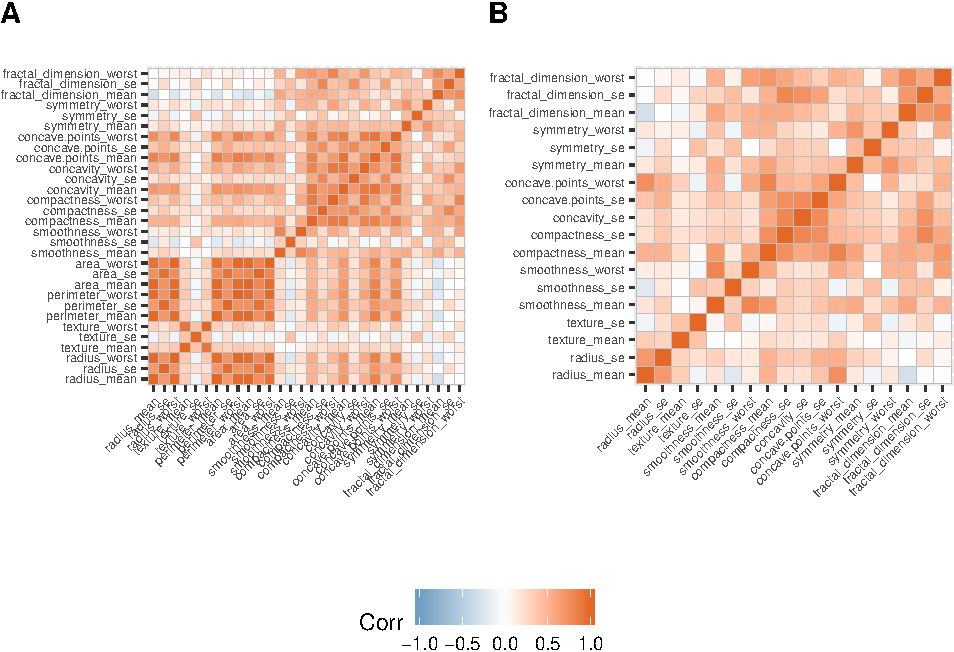
\includegraphics{test_files/figure-beamer/unnamed-chunk-1-1.pdf}

\end{frame}

\begin{frame}{Logistic Model with Newton-Raphson}

\textbf{Logistic Regression:}

\(y\): the vector of \(n\) response random variable

\(X\): the \(n\times p\) design matrix (\(X_{i}\) denote the \(i\)th
row)

\(\beta\): the \(p\times 1\) coefficient

\begin{itemize}
\tightlist
\item
  The logistic regression model:
\end{itemize}

\[\log(\frac{\eta}{1-\eta}) = X\beta\]

\begin{itemize}
\tightlist
\item
  The likelihood function:
\end{itemize}

\[L(\beta; X, y) = \prod_{i=1}^n \{(\frac{\exp(X_{i}\beta)}{1+\exp(X_{i}\beta)})^{y_i}(\frac{1}{1+\exp(X_{i}\beta)})^{1-y_i}\}\]

\end{frame}

\begin{frame}{}

\begin{itemize}
\item
  The log likelihood: \[
  \begin{aligned}
  l(\beta) 
  & = \sum_{i=1}^n \{y_i(X_{i}\beta)-\log(1+\exp(X_{i}\beta))\}
  \end{aligned}
  \]
\item
  The gradient: \[
  \nabla l(\beta) = X^T(y-p)
  \] where \(p=\frac{\exp(X\beta)}{1+\exp(X\beta)}\)
\item
  The Hessian: \[
  \nabla^2 l(\beta) = -X^T W X
  \] where \(W = diag(p_i(1-p_i)), i=1,\cdots,n\). The Hessian is
  negative definite.
\end{itemize}

\end{frame}

\begin{frame}{}

\textbf{Newton-Raphson}

\emph{Update coefficients}
\[\beta_{i+1} = \beta_{i} -[\nabla^2 l(\beta_{i})]^{-1}\nabla l(\beta_{i})\]
\emph{Step-halving} \[
\beta_{i+1}(\gamma) = \beta_{i} - \gamma[\nabla^2 l(\beta_{i})]^{-1}\nabla l(\beta_{i})
\]

\begin{itemize}
\tightlist
\item
  Set \(\gamma = 1\)
\item
  If \(f(\theta_{i+1}(1)) \geq f(\theta_{i})\), then set
  \(\theta_{i+1} = \theta_{i+1}(1)\)
\item
  If \(f(\theta_{i+1}(1)) \leq f(\theta_{i})\), search for a value
  \(\gamma \in (0,1)\) for which
  \(f(\theta_{i+1}(\gamma)) \geq f(\theta_{i})\), set
  \(\theta_{i+1} = \theta_{i+1}(\gamma)\)
\end{itemize}

\end{frame}

\begin{frame}{}

\textbf{Newton-Raphson: gradient decent}

For Newton's method with a large \(p\), the computational burden in
calculating the inverse of the Hessian Matrix
\([\nabla^2 f(\beta_{i})]^{-1}\) increases quickly with \(p\). One can
update \[
\beta_{i+1} = \beta_{i} + H_{i}\nabla f(\beta_{i})
\] where \(H_{i} = (X^TX)^{-1}\) for every \(i\). This is easy to
compute, but could be slow in convergence.

The steps are:

\begin{itemize}
\tightlist
\item
  get the objective (loglik,grad,Hess) function
\item
  use the principle of newton raphson to update the estimate, if the
  step size too large, step-halving step
\item
  stop searching until the convergences of the estimates.
\end{itemize}

\end{frame}

\begin{frame}{Logistic-LASSO Model with Pathwise Coordinate Descent}

\begin{itemize}
\item
  Applied coordinate-wise descent with weighted update: \[
  \tilde{\beta}^{lasso}_{j}(\lambda) \leftarrow \frac{S(\sum_{i=1}^{n}\omega_{i}x_{i,j}(y_{i} - \tilde{y_{i}}^{(-j)}), \lambda)}{\sum_{i=1}^n\omega_{i}x_{i,j}^{2}}
  \] where
  \(\tilde{y_{i}}^{(-j)} = \sum_{k \neq j}x_{i,k}\tilde{\beta_{k}}\) and
  \(S(\hat{\beta}, \lambda) = sign(\hat{\beta})(|\hat{\beta}| - \lambda)_{+}\)
\item
  In the context of logistic regression, we are aiming to maximize the
  penalized log likelihood:
  \[\max_{\beta \in \mathbb{R}^{p+1}} \frac{1}{n}\sum_{i=1}^n  \{y_i(X_{i}\beta)-\log(1+\exp(X_{i}\beta))\}-\lambda \sum_{j=0}^p |\beta_j|\]
  for some \(\lambda \geq 0\)
\end{itemize}

\end{frame}

\begin{frame}{Result}

\textbf{Estimation Path}

\includegraphics{test_files/figure-beamer/unnamed-chunk-3-1.pdf}

\end{frame}

\begin{frame}{}

\textbf{Cross validation for LASSO}

\includegraphics{test_files/figure-beamer/unnamed-chunk-4-1.pdf}

\end{frame}

\begin{frame}{}

\textbf{Model Comparison}

\begin{table}[!h]

\caption{\label{tab:unnamed-chunk-5}The comparison of performance for estimation algorithms and models}
\centering
\resizebox{\linewidth}{!}{
\begin{tabular}{llllll}
\toprule
  & GLM package & Newton Raphson & Gradient Decent & Logistic Lasso & Lasso package\\
\midrule
iteration times & NA & 12 & 1001 & 100 & NA\\
MSE & 0.02 & 0.02 & 0.02 & 0.02 & 0.02\\
\bottomrule
\multicolumn{6}{l}{\textsuperscript{a} Dataset: Breast Cancer Diagnosis}\\
\end{tabular}}
\end{table}

\end{frame}

\end{document}
